%%%%%%%%%%%%%%%%%%%%%%%%%%%%%%%%%%%%%%%%%%%%%%%%%%%%%%%%%%%%%%%%%%%%%%%%
% Preamble
%%%%%%%%%%%%%%%%%%%%%%%%%%%%%%%%%%%%%%%%%%%%%%%%%%%%%%%%%%%%%%%%%%%%%%%%
\documentclass[12pt]{article}
%
% Packages and other includes
% Pagination
\usepackage[letterpaper, margin=1in]{geometry}

%
% Graphics, floats, tables
\usepackage{graphicx, xcolor, float, array}
\graphicspath{{image/}}
%
% Fonts
\usepackage[T1]{fontenc} % best for Western European languages
\usepackage{lmodern} % Latin Modern instead of CM
\usepackage{textcomp} % required to get special symbols
%
% Math
\usepackage{amsmath, amssymb}
\usepackage{enumerate}
\usepackage{braket}
% 
% Hyperlinks
\usepackage[colorlinks,linkcolor={red},citecolor={blue},
urlcolor={blue}]{hyperref} 
%
% Definitions and settings
% Paragraph indent and spacing
\setlength{\parskip}{0.4\baselineskip}
\setlength{\parindent}{0in}
%
% Math mode version of "r" column type (requires array package)
\newcolumntype{R}{>{$}r<{$}}
\newcommand{\brian}[1]{{\color{orange}{#1}}}
% Title, authors, date
\title{\textbf{Homework 7}}
\date{\vspace{-2em}\today}

\begin{document}

\maketitle 

Weekly homework assignments are posted approximately one week prior to the
due date. Collaborations are encouraged and students must report all collaborators
in writing on each assignment. All external sources (websites, books) must be
properly cited. Additional problems are listed at the end of each assignment.
This week's assignment is due \textit{Friday, Oct 21st at 11:59pm.}

\textbf{Conservation of Energy}

1. Consider two isolated systems containing water illustrated below. The system on the left is
at $100^\circ\text{C}$ and the other (right) is at room temperature of $20^\circ\text{C}$. The
isolated systems are allowed to come into contact reaching thermal equilibrium and without losing
energy to the surrounding. What is the final temperature? Describe in words, mathematical
equations and/or illustrations what happened. (2 pts)

\begin{center}
  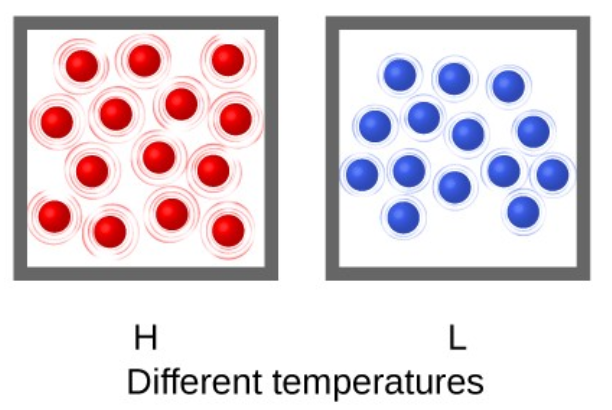
\includegraphics[scale=0.25]{isolated_sys.png}
\end{center}


\newpage

2. Suppose a system is in thermal equilibrium with a heat bath (source of heat that
maintains at a constant temperature). Suppse the temperature of the heat bath increases,
describe in words and/or illustrations what happens to the temperature of the system. (2 pts)

\vspace{2.5in}



\textbf{Limiting Reagent}

3. For the complete combustion of liquid propanol (C$_3$H$_7$OH), it produces gaseous
carbon dioxide (CO$_2$) and water (H$_2$O).

a) Write the balanced and complete chemical equation.

b) Suppose there is 10.g CH$_3$H$_7$OH and 10.g O$_2$ available. Which is the limiting
reagent? And how much CO$_2$ is produced in g? Report to 2 significant figures.

\newpage

4. An important step in the refining of aluminum metal is the manufacture of cryolite,
Na$_3$AlF$_6$, from ammonium fluoride, sodium aluminate, and sodium hydroxide in aqueous
solution:

6NH$_4$F(aq) + Na[Al(OH)$_4$](aq) + 2NaOH(aq) $\rightarrow$ Na$_3$AlF$_6$(s) + 6NH$_3$(aq)
+ 6H$_2$O(l)

Unfortunately, by-products can form, reducing the yield. In a laboratory investigation of
the process, 100.0g of NH$_4$F was mixed with 82.60g of Na[Al(OH)$_4$] and 80.00g of NaOH.
The mass of Na$_3$AlF$_6$ produced was 75.00g. What was the percentage yield of the reaction?
Report to 4 significant figures. (3 pts)

\vspace{3in}

\textbf{Energy Changes}

5. How much heat has to be added to 250g solid Fe at 22.5$^\circ$C to raise the temperature to
250$^\circ$C? The specific heat of solid Fe is 0.448 J/(g $^\circ$C). Report to 3 significant
figures (1 pt)

\vfill

\textbf{Optional Textbook Problems:} Ch. 6- $6.29 - 6.49$ odd, $6.63 - 6.93$

\end{document}
